\documentclass{standalone}
\usepackage{pgfplots}
\makeatletter
\let\originalfinalscales\pgfplots@scaling@compute@final@scales
\def\pgfplots@scaling@compute@final@scales#1#2#3#4#5{%
  \typeout{SCALE input x=#1 y=#2 inv=#3,#4,#5}%
  \typeout{SCALE basis x=\the\pgf@xx,\the\pgf@xy; y=\the\pgf@yx,\the\pgf@yy; z=\the\pgf@zx,\the\pgf@zy}%
  \typeout{SCALE limits x=\pgfplots@xmin,\pgfplots@xmax; y=\pgfplots@ymin,\pgfplots@ymax; z=\pgfplots@zmin,\pgfplots@zmax}%
  \originalfinalscales{#1}{#2}{#3}{#4}{#5}%
  \typeout{SCALE output xx=\pgfplots@target@unit@scale@xx xy=\pgfplots@target@unit@scale@xy yx=\pgfplots@target@unit@scale@yx yy=\pgfplots@target@unit@scale@yy zx=\pgfplots@target@unit@scale@zx zy=\pgfplots@target@unit@scale@zy}%
}
\newcommand{\extent}{\coordinate (lo) at (axis description cs:0,0);\coordinate (hi) at (axis description cs:1,1);
\coordinate (b0) at (rel axis cs:0,0,0);\coordinate (bx) at (rel axis cs:1,0,0);\coordinate (by) at (rel axis cs:0,1,0);\coordinate (bz) at (rel axis cs:0,0,1);}
\newcommand{\reportextent}{\pgfextractx{\dimen0}{\pgfpointdiff{\pgfpointanchor{lo}{center}}{\pgfpointanchor{hi}{center}}}\pgfextracty{\dimen2}{\pgfpointdiff{\pgfpointanchor{lo}{center}}{\pgfpointanchor{hi}{center}}}\typeout{EXTENT \the\dimen0,\the\dimen2}
\foreach \v in {bx,by,bz}{\pgfextractx{\dimen0}{\pgfpointdiff{\pgfpointanchor{b0}{center}}{\pgfpointanchor{\v}{center}}}\pgfextracty{\dimen2}{\pgfpointdiff{\pgfpointanchor{b0}{center}}{\pgfpointanchor{\v}{center}}}\typeout{BASIS \v: \the\dimen0,\the\dimen2}}}
\makeatother
\begin{document}
\typeout{CASE default}
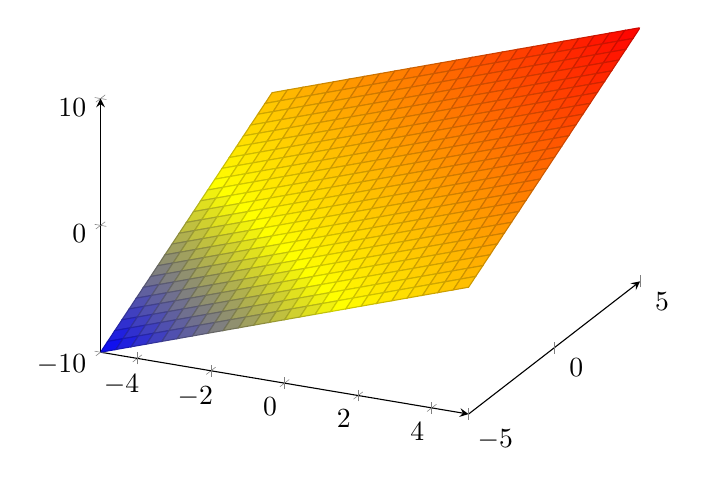
\begin{tikzpicture}
\begin{axis}[axis lines=left]
\addplot3[surf] {x+y};
\extent
\end{axis}
\reportextent
\end{tikzpicture}
\typeout{CASE modern}
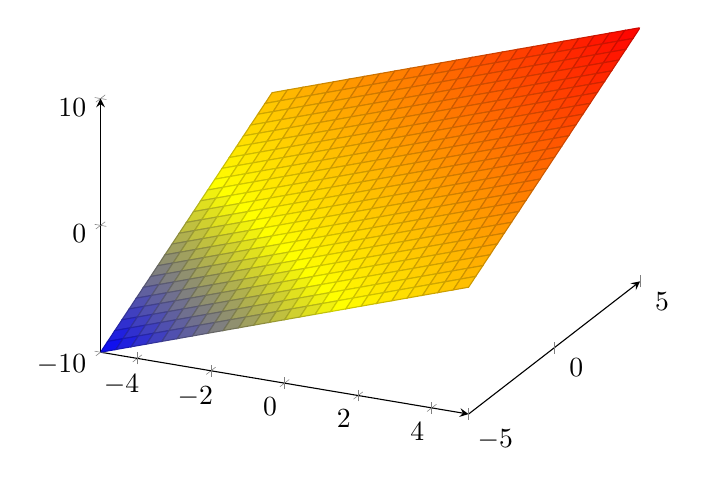
\begin{tikzpicture}
\begin{axis}[compat=1.18,axis lines=left]
\addplot3[surf] {x+y};
\extent
\end{axis}
\reportextent
\end{tikzpicture}
\typeout{CASE compat13}
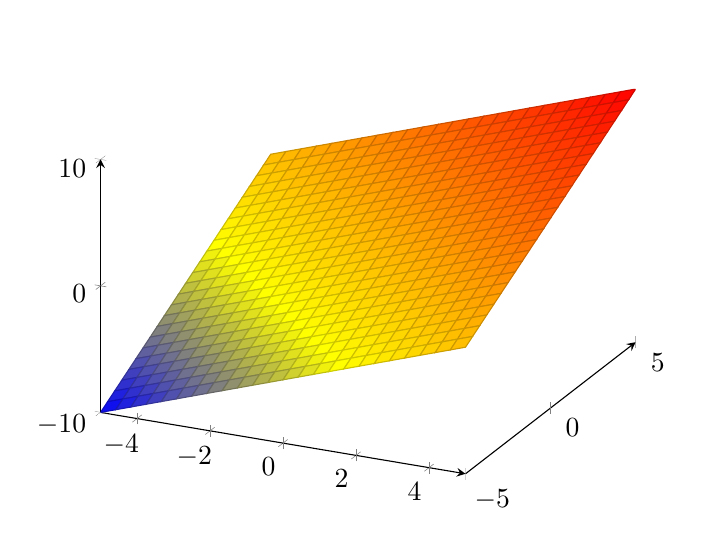
\begin{tikzpicture}
\begin{axis}[compat=1.3,axis lines=left]
\addplot3[surf] {x+y};
\extent
\end{axis}
\reportextent
\end{tikzpicture}
\typeout{CASE ridge}
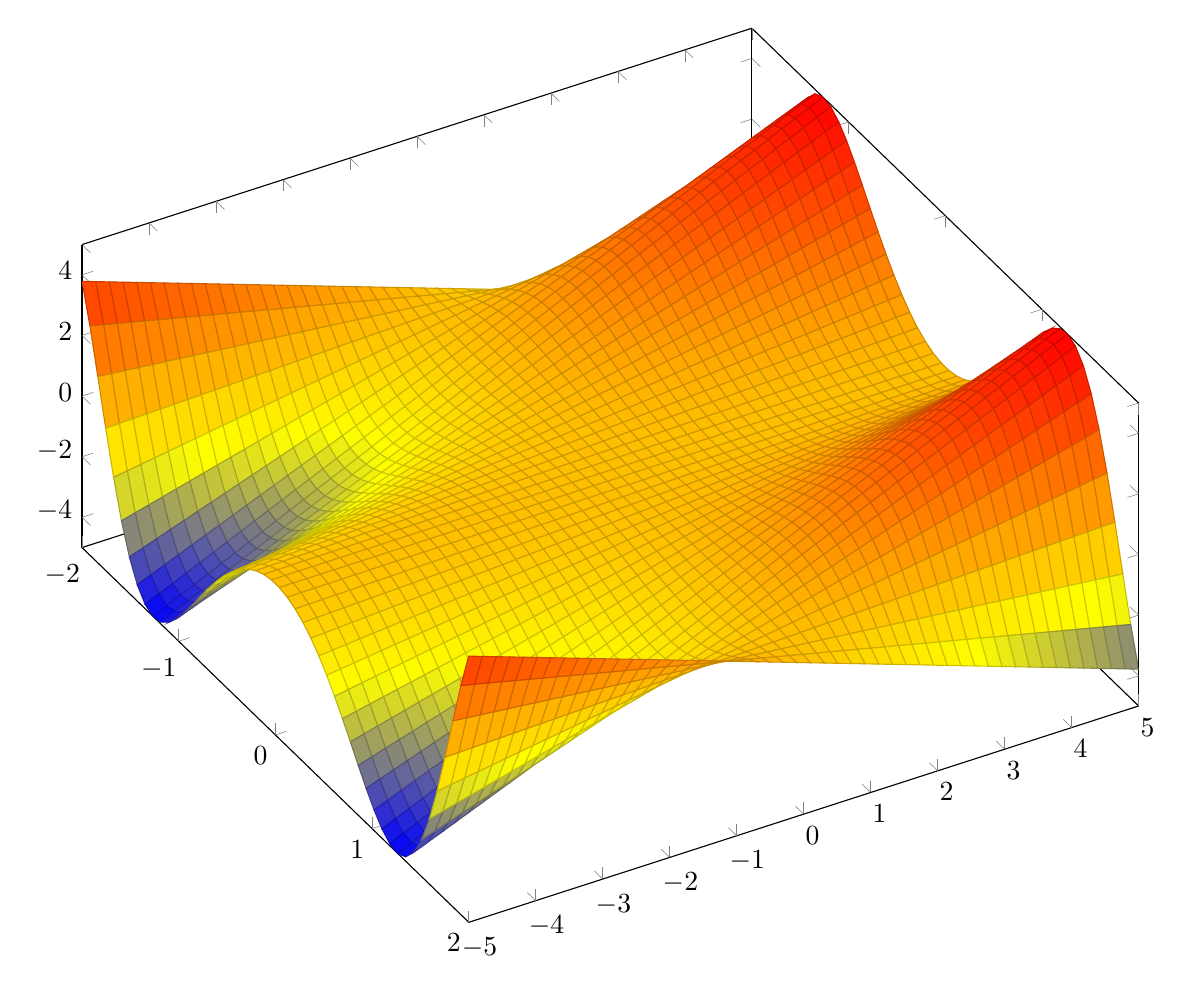
\begin{tikzpicture}
\begin{axis}[width=15cm,view={60}{55},enlargelimits=false,domain=-2:2,y domain=-5:5,samples=50]
\addplot3[surf] {sin((x*x)r)*y};
\extent
\end{axis}
\reportextent
\end{tikzpicture}
\typeout{CASE function4}
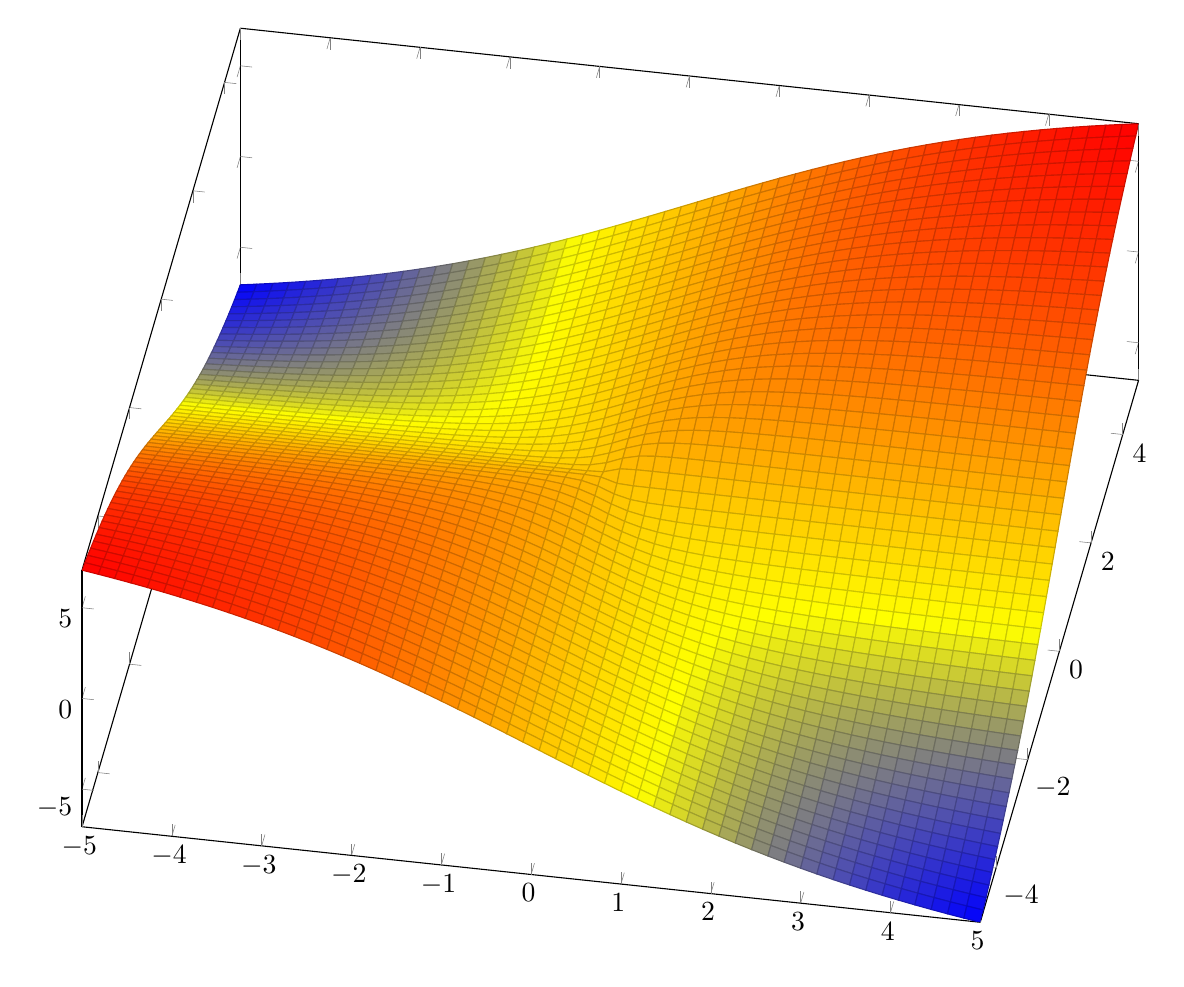
\begin{tikzpicture}
\begin{axis}[width=15cm,view={10}{65},enlargelimits=false,domain=-5:5,y domain=-5:5,samples=56]
\addplot3[surf] {2*x*y/sqrt(x*x+y*y)};
\extent
\end{axis}
\reportextent
\end{tikzpicture}
\typeout{CASE compact}
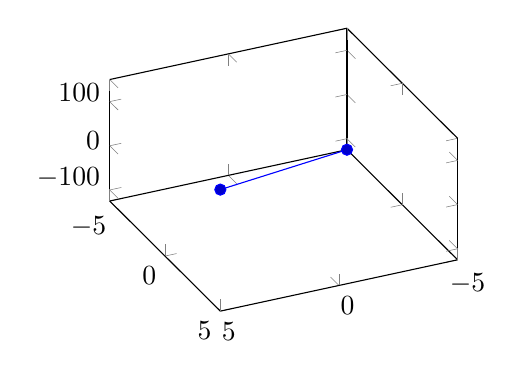
\begin{tikzpicture}
\begin{axis}[width=6cm,view={155}{45},xmin=-5,xmax=5,ymin=-5,ymax=5,zmin=-125,zmax=150,enlargelimits=false]
\addplot3 coordinates {(-5,-5,-125) (5,5,150)};
\extent
\end{axis}
\reportextent
\end{tikzpicture}
\typeout{CASE ratio}
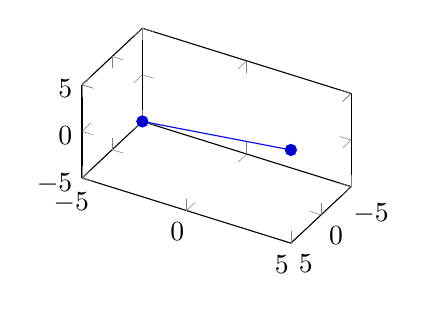
\begin{tikzpicture}
\begin{axis}[width=5cm,view={120}{35},plot box ratio={1}{2}{1},xmin=-5,xmax=5,ymin=-5,ymax=5,zmin=-5,zmax=5,enlargelimits=false]
\addplot3 coordinates {(-5,-5,-5) (5,5,5)};
\extent
\end{axis}
\reportextent
\end{tikzpicture}
\typeout{CASE compact15}
\begin{tikzpicture}
\begin{axis}[width=15cm,view={65}{65},xmin=-5,xmax=5,ymin=-5,ymax=5,zmin=-125,zmax=150,enlargelimits=false]
\addplot3 coordinates {(-5,-5,-125) (5,5,150)};
\extent
\end{axis}\reportextent
\end{tikzpicture}
\typeout{CASE default-fixed}
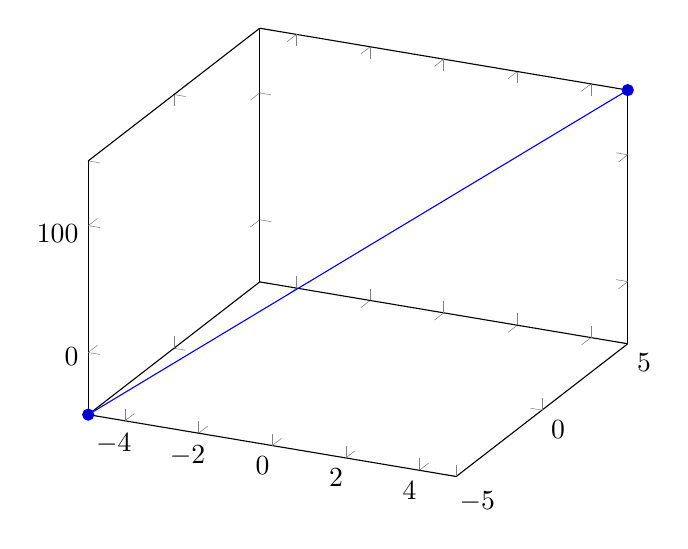
\begin{tikzpicture}
\begin{axis}[xmin=-5,xmax=5,ymin=-5,ymax=5,zmin=-49,zmax=151,enlargelimits=false]
\addplot3 coordinates {(-5,-5,-49) (5,5,151)};
\extent
\end{axis}\reportextent
\end{tikzpicture}
\typeout{CASE explicit45}
\begin{tikzpicture}
\begin{axis}[width=15cm,view={45}{45},xmin=-90,xmax=90,ymin=-90,ymax=90,zmin=-4,zmax=4,enlargelimits=false]
\addplot3 coordinates {(-90,-90,-4) (90,90,4)};
\extent
\end{axis}\reportextent
\end{tikzpicture}
\foreach \w in {5cm,8cm}{\foreach \r in {1,2}{
\typeout{CASE equal-ratio width=\w ratio=\r}
\begin{tikzpicture}
\begin{axis}[width=\w,view={25}{30},plot box ratio={\r}{\r}{\r},xmin=0,xmax=1,ymin=0,ymax=1,zmin=0,zmax=1,enlargelimits=false]
\addplot3 coordinates {(0,0,0) (1,1,1)};
\extent
\end{axis}\reportextent
\end{tikzpicture}}}
\typeout{CASE auto-z}
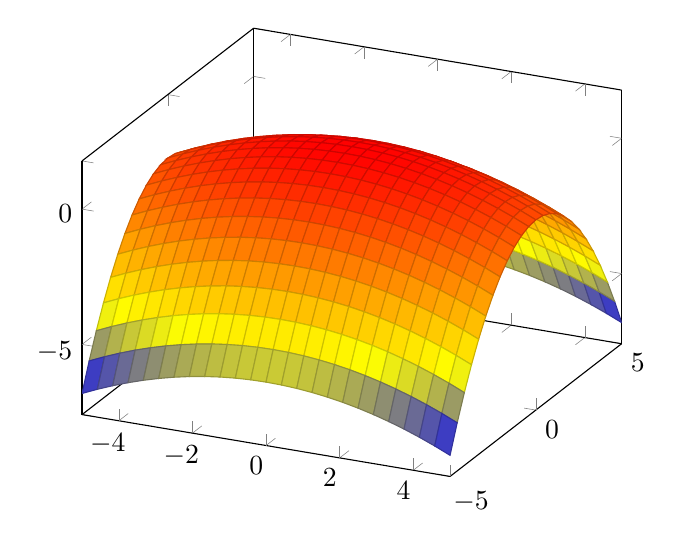
\begin{tikzpicture}
\begin{axis}
\addplot3[surf] {-(x*x/16+y*y/4-1)};
\extent
\end{axis}\reportextent
\end{tikzpicture}
\end{document}
